\documentclass[11pt,a4paper]{article}
\usepackage[margin=2cm]{geometry}
\usepackage{graphicx}
\usepackage{amsmath,amssymb}
\usepackage{enumitem}
\usepackage{xcolor}
\usepackage{tcolorbox}
\usepackage{booktabs}
\usepackage{hyperref}
\usepackage{fancyhdr}

\definecolor{qcolor}{HTML}{1A5276}
\definecolor{acolor}{HTML}{196F3D}
\definecolor{boxbg}{HTML}{EBF5FB}
\definecolor{ansbox}{HTML}{EAFAF1}
\definecolor{tipbox}{HTML}{FEF9E7}

\tcbset{
    qbox/.style={colback=boxbg, colframe=qcolor, coltitle=white, fonttitle=\bfseries, coltext=black, left=4pt, right=4pt, top=4pt, bottom=4pt, boxrule=0.8pt, arc=3pt},
    abox/.style={colback=ansbox, colframe=acolor, coltitle=white, fonttitle=\bfseries, coltext=black, left=4pt, right=4pt, top=4pt, bottom=4pt, boxrule=0.5pt, arc=3pt},
    tipbox/.style={colback=tipbox, colframe=orange!70!black, fonttitle=\bfseries, left=4pt, right=4pt, top=4pt, bottom=4pt, boxrule=0.5pt, arc=3pt}
}

\newcounter{qcounter}
\setcounter{qcounter}{34}
\newcommand{\vq}[1]{\stepcounter{qcounter}\begin{tcolorbox}[qbox, title=Q\theqcounter]#1\end{tcolorbox}}
\newcommand{\va}[1]{\begin{tcolorbox}[abox, title=Answer]#1\end{tcolorbox}\vspace{6pt}}

\pagestyle{fancy}
\fancyhf{}
\fancyhead[L]{\small\textbf{TFML Viva Prep — Part 2}}
\fancyhead[R]{\small CS6302E | Winter 2026}
\fancyfoot[C]{\thepage}

\title{\textbf{TFML Assignment Viva — Question Bank}\\[4pt]\Large Part 2: Backpropagation, Confusion Matrix \& Weight Visualization}
\author{CS6302E — Theoretical Foundations of Machine Learning}
\date{NIT Calicut | Winter 2026}

\begin{document}
\maketitle
\tableofcontents
\newpage

%=============================================================================
\section{Backpropagation — The Math}
%=============================================================================

\vq{Derive the backpropagation equations for your network.}
\va{For MSE loss with sigmoid, forward pass:
$z_1 = XW_1 + b_1$, $a_1 = \sigma(z_1)$; \quad $z_2 = a_1W_2 + b_2$, $a_2 = \sigma(z_2)$; \quad $L = \frac{1}{n}\sum(y - a_2)^2$

\textbf{Output layer:}
\begin{align*}
    \delta_2 &= (a_2 - y) \cdot \sigma'(z_2) = (a_2 - y) \cdot a_2(1 - a_2) \\
    \frac{\partial L}{\partial W_2} &= \frac{1}{n} a_1^T \cdot \delta_2, \quad
    \frac{\partial L}{\partial b_2} = \frac{1}{n} \sum \delta_2
\end{align*}

\textbf{Hidden layer (chain rule):}
\begin{align*}
    \delta_1 &= (\delta_2 \cdot W_2^T) \cdot a_1(1 - a_1) \\
    \frac{\partial L}{\partial W_1} &= \frac{1}{n} X^T \cdot \delta_1, \quad
    \frac{\partial L}{\partial b_1} = \frac{1}{n} \sum \delta_1
\end{align*}
}

\vq{Why do we multiply by the sigmoid derivative during backpropagation?}
\va{Because of the \textbf{chain rule}: $\frac{\partial L}{\partial z_2} = \frac{\partial L}{\partial a_2} \cdot \frac{\partial a_2}{\partial z_2}$. The second factor is $\sigma'(z_2) = a_2(1-a_2)$. It tells us how much a small change in pre-activation $z$ affects the output $a$.}

\vq{How does the gradient flow backward from output to hidden layer?}
\va{$\delta_1 = (\delta_2 \cdot W_2^T) \cdot a_1(1-a_1)$
\begin{itemize}[nosep]
    \item $\delta_2 \cdot W_2^T$: Output error is \textbf{projected back} through transpose of $W_2$, distributing blame to each hidden unit proportional to its weight
    \item Multiply by $a_1(1-a_1)$: Scales by the \textbf{local sigmoid derivative}, accounting for each hidden neuron's responsiveness
\end{itemize}
}

\vq{What is the gradient descent update rule?}
\va{$W \leftarrow W - \eta \cdot \frac{\partial L}{\partial W}$

The weight is adjusted in the \textbf{negative gradient direction} (steepest descent). The learning rate $\eta$ controls the step size.}

\vq{Why do you divide the gradient by n\_samples?}
\va{Because we use \textbf{Mean} Squared Error. Dividing by $n$ ensures the gradient magnitude is \textbf{independent of dataset size}, so the learning rate doesn't need adjustment when the dataset size changes.}

\vq{What is the computational complexity of one training epoch?}
\va{For a $64\text{-}X\text{-}3$ network with $N$ samples:
\begin{itemize}[nosep]
    \item Forward: $O(N \cdot 64 \cdot X) + O(N \cdot X \cdot 3)$
    \item Backward: Same order (symmetric matrix multiplications)
    \item For 64-3-3 with 300 samples: $\sim$300 $\times$ 207 $\approx$ 62,100 multiply-adds per epoch
\end{itemize}
}

\vq{What is the difference between full-batch, mini-batch, and stochastic GD?}
\va{
\begin{center}
\begin{tabular}{lccc}
\toprule
\textbf{Method} & \textbf{Batch Size} & \textbf{Gradient} & \textbf{Noise} \\
\midrule
Full-batch GD (ours) & All $N=300$ & Exact & None \\
Mini-batch GD & $k$ (e.g.\ 32) & Approximate & Some \\
Stochastic GD & 1 & Very noisy & High \\
\bottomrule
\end{tabular}
\end{center}
We used full-batch because with 300 samples, computing the exact gradient is cheap and gives stable, monotonic convergence.
}

%=============================================================================
\section{Confusion Matrix Analysis}
%=============================================================================

\vq{Explain the confusion matrix from your 64-3-3 network.}
\va{
\begin{center}
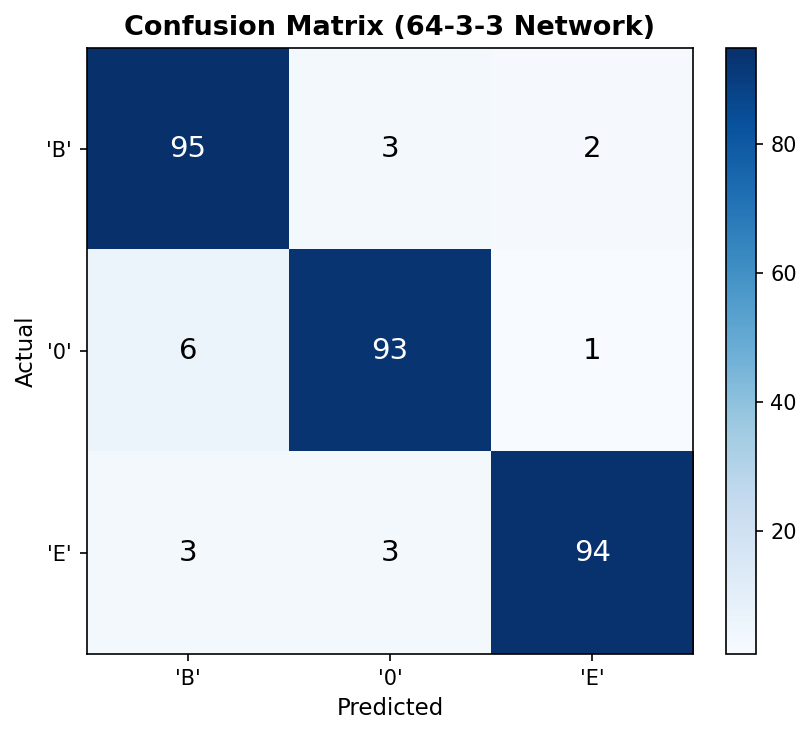
\includegraphics[width=0.45\textwidth]{confusion_matrix.png}
\end{center}

\begin{center}
\begin{tabular}{lccc}
\toprule
& \textbf{Pred B} & \textbf{Pred 0} & \textbf{Pred E} \\
\midrule
\textbf{Actual B} & \textbf{95} & 3 & 2 \\
\textbf{Actual 0} & 6 & \textbf{93} & 1 \\
\textbf{Actual E} & 3 & 3 & \textbf{94} \\
\bottomrule
\end{tabular}
\end{center}
Diagonal = correct: $95 + 93 + 94 = 282/300 = \mathbf{94\%}$. Off-diagonal = 18 errors.
}

\vq{Which pair of letters is most confused and why?}
\va{\textbf{B and 0} are most confused (9 total cross-misclassifications). Both share: vertical bars on the left side, enclosed regions, similar top/bottom edges. The main difference is the \textbf{middle horizontal bar} in B. Heavy noise on middle-row pixels makes this distinction unreliable.}

\vq{What is the per-class precision, recall, and F1?}
\va{
\begin{itemize}[nosep]
    \item \textbf{B}: Precision $= 95/104 = 91.3\%$, Recall $= 95/100 = 95\%$, F1 $= 93.1\%$
    \item \textbf{0}: Precision $= 93/99 = 93.9\%$, Recall $= 93/100 = 93\%$, F1 $= 93.5\%$
    \item \textbf{E}: Precision $= 94/97 = 96.9\%$, Recall $= 94/100 = 94\%$, F1 $= 95.4\%$
\end{itemize}
E has the highest precision because its structure (open right side) is most distinctive.
}

\vq{Why are some misclassifications unavoidable?}
\va{With noise in $[-5, +5]$ and signal in $[-1, +1]$, some noisy samples will be \textbf{closer to a different letter's template} than their own. These are \textbf{Bayes-irreducible errors} — no classifier can get them right. The $\sim$6\% error rate approximates the \textbf{Bayes error rate} for this noise level.}

%=============================================================================
\section{Input-to-Hidden Weight Visualization (Part b)}
%=============================================================================

\vq{What do the input-to-hidden weight visualizations show?}
\va{
\begin{center}
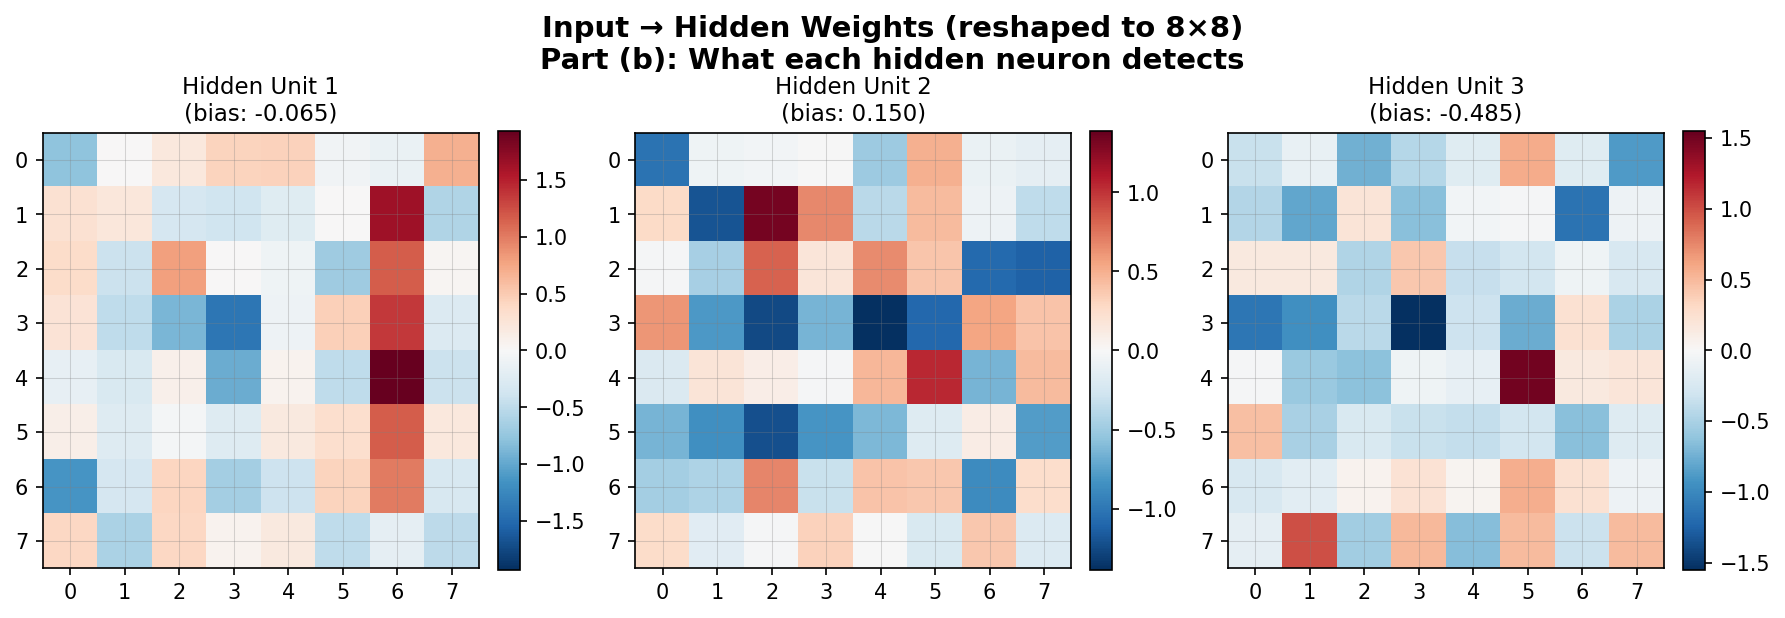
\includegraphics[width=0.85\textwidth]{input_hidden_weights.png}
\end{center}
Each hidden unit has 64 weights connecting it to the 64 input pixels. These are \textbf{reshaped into $8\times 8$ images}. \textbf{Red = positive weights} (activates when pixel is white/$+1$), \textbf{Blue = negative weights} (activates when pixel is black/$-1$).
}

\vq{How do you interpret the weight images? What is each hidden neuron detecting?}
\va{Each hidden neuron's weight image acts as a \textbf{matched filter / template detector}:
\begin{itemize}[nosep]
    \item When input \textbf{aligns} with the weight pattern, the dot product is maximized $\to$ neuron fires strongly
    \item When input \textbf{opposes} the weight pattern, dot product is minimized $\to$ neuron stays inactive
    \item The 3 hidden neurons detect \textbf{different distinguishing features}: right-side openness (E vs B/0), middle bar (B/E vs 0), enclosure (0/B vs E)
\end{itemize}
}

\vq{Why do the weight patterns look like blurry versions of the letters?}
\va{Because noise has zero mean, after averaging across 100 training samples, the noise cancels and weights reflect the \textbf{underlying template structure}. The ``blur'' comes from each neuron detecting a \textbf{distinguishing feature} that separates classes, not a single letter.}

\vq{What do the bias values (HU1: $-0.065$, HU2: $+0.150$, HU3: $-0.485$) mean?}
\va{The bias shifts the \textbf{activation threshold}:
\begin{itemize}[nosep]
    \item HU1 ($-0.065$): Nearly zero — balanced detector
    \item HU2 ($+0.150$): Small positive — slightly easier to activate (lower threshold)
    \item HU3 ($-0.485$): Significant negative — \textbf{harder to activate}, requires stronger positive input. Detects a more selective feature.
\end{itemize}
}

\vq{Explain the connection between each hidden neuron and the dot product operation.}
\va{The hidden layer computes: $z_j = \sum_{i=1}^{64} w_{ij} \cdot x_i + b_j$

This is a \textbf{dot product} between weight vector and input vector, plus bias. Geometrically, it measures \textbf{cosine similarity} (scaled) between input and the weight pattern. High dot product = input is ``similar'' to the weight pattern $\to$ neuron fires. This is why weight images look like the features the neuron ``looks for.''}

\vq{If you had only 2 hidden neurons instead of 3, what would the weight images look like?}
\va{With 2 hidden neurons for 3 classes, the network creates a \textbf{2D embedding}. Weight images would represent \textbf{combined features} (e.g., one neuron for ``has middle bar'' separating B+E from 0, another for ``has right side'' separating B+0 from E), but the network would likely fail on some class — underdetermined.}

%=============================================================================
\section{Hidden-to-Output Weight Visualization (Part c)}
%=============================================================================

\vq{What do the hidden-to-output weights represent?}
\va{
\begin{center}
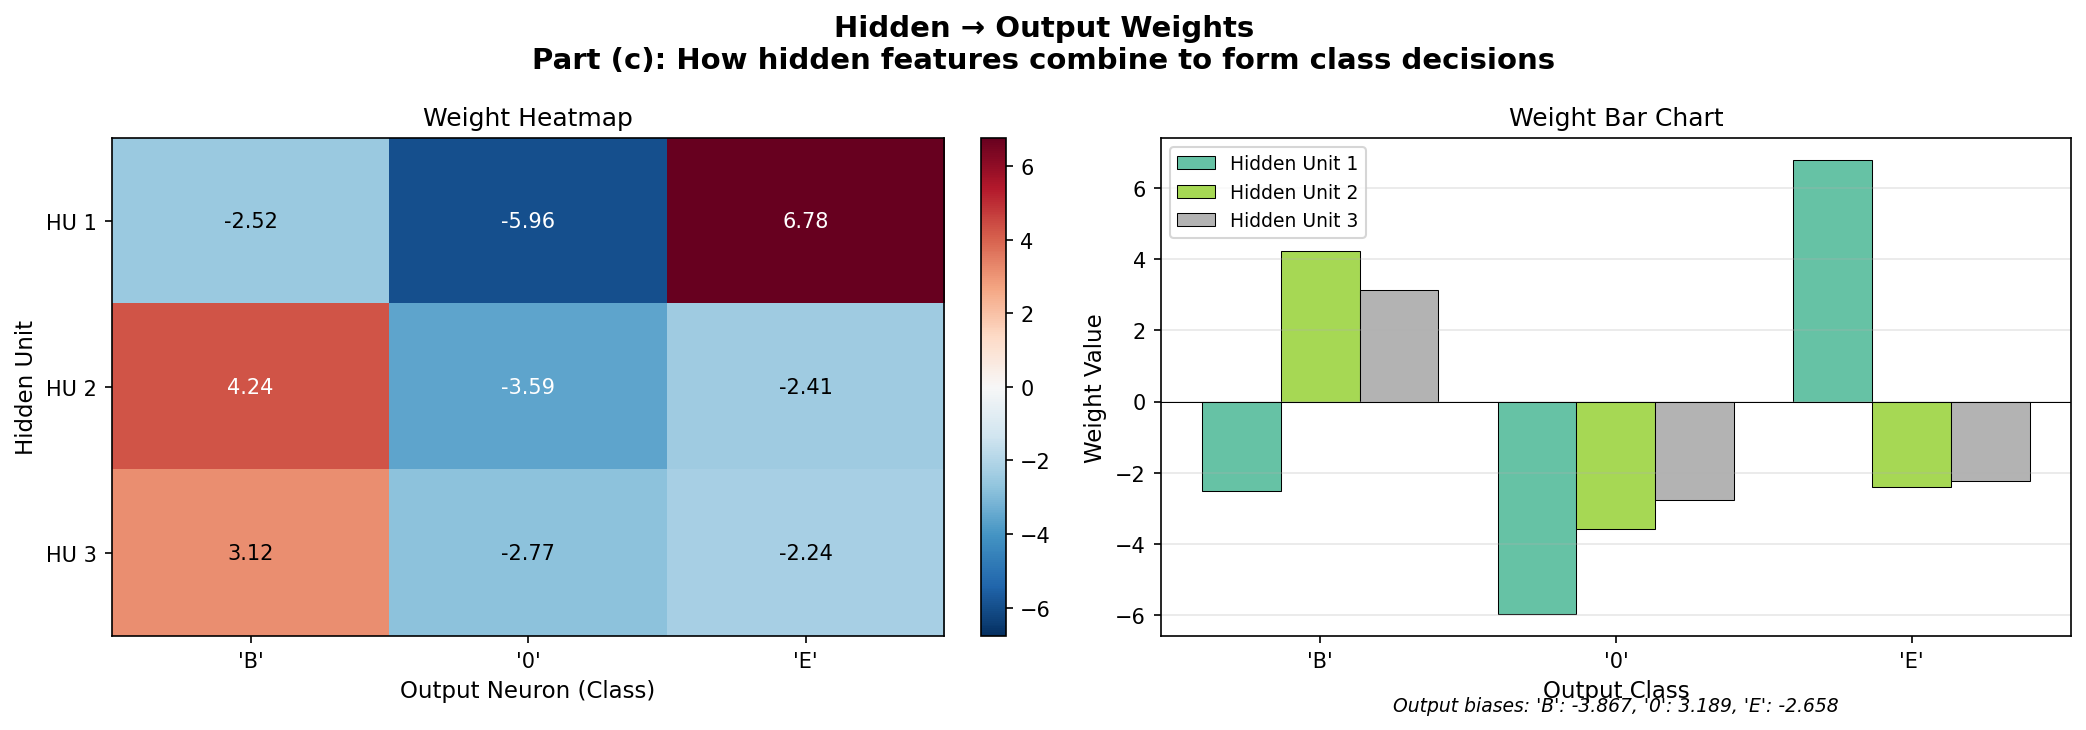
\includegraphics[width=0.90\textwidth]{hidden_output_weights.png}
\end{center}
A \textbf{$3\times 3$ matrix} connecting hidden units to output neurons. Each weight determines \textbf{how strongly} a hidden unit's activation supports or opposes a particular class. Positive (red) = supports; negative (blue) = opposes.
}

\vq{Read the heatmap values and explain the classification logic.}
\va{
\begin{center}
\begin{tabular}{lccc}
\toprule
& \textbf{B output} & \textbf{0 output} & \textbf{E output} \\
\midrule
\textbf{HU1} & $-2.52$ & $-5.96$ & $\mathbf{+6.78}$ \\
\textbf{HU2} & $\mathbf{+4.24}$ & $-3.59$ & $-2.41$ \\
\textbf{HU3} & $\mathbf{+3.12}$ & $-2.77$ & $-2.24$ \\
\bottomrule
\end{tabular}
\end{center}
\begin{itemize}[nosep]
    \item \textbf{Class E} relies on HU1 ($+6.78$) — when HU1 fires, predict E
    \item \textbf{Class B} relies on HU2 ($+4.24$) and HU3 ($+3.12$) — both must fire for B
    \item \textbf{Class 0} has all negative weights — predicted when \textbf{none} fire strongly
\end{itemize}
This creates a \textbf{combinatorial code}: 3 hidden activations form a unique signature per class.
}

\vq{What are the output biases and what role do they play?}
\va{Biases: B $= -3.867$, 0 $= +3.189$, E $= -2.658$.
\begin{itemize}[nosep]
    \item \textbf{0 has large positive bias ($+3.189$)}: Default prediction when hidden units are inactive — aligns with all-negative weights for 0
    \item \textbf{B and E have negative biases}: Need strong positive hidden input to overcome the negative bias
    \item Biases encode the network's \textbf{prior/default preference} before seeing evidence
\end{itemize}
}

\vq{How does the two-layer decision process work conceptually?}
\va{Two-stage decision:
\begin{enumerate}[nosep]
    \item \textbf{Feature extraction} (input$\to$hidden): Each hidden neuron computes a dot product, acting as a feature detector (``is the right side open?'', ``is there a middle bar?'')
    \item \textbf{Feature-based decision} (hidden$\to$output): Output layer combines detected features. Each class has a unique ``recipe'' of required features.
\end{enumerate}
Analogous to how a human classifies: first identify structural elements, then match the combination to a known letter.
}

\begin{tcolorbox}[tipbox, title=\textbf{End of Part 2}]
\textbf{21 questions (Q35--Q55) covered.} Continue to Part 3 for architecture search, sample complexity, and generalization theory.
\end{tcolorbox}

\end{document}
